\section{Experimental setup}
\label{sec:setup}

\begin{figure}[t]
  \centering
  \begin{minipage}[b]{0.48\linewidth}
    \centering
    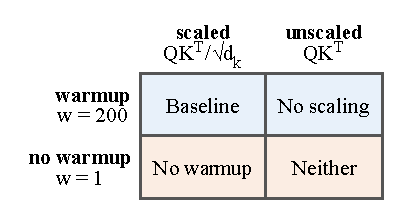
\includegraphics[width=\linewidth]{figures/ablation_grid.pdf}
  \end{minipage}\hfill
  \begin{minipage}[b]{0.48\linewidth}
    \centering
    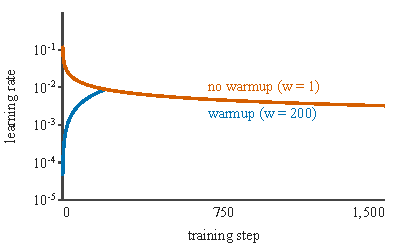
\includegraphics[width=\linewidth]{figures/lr_schedule_concept.pdf}
  \end{minipage}
  \caption{The ablation crosses warmup with attention scaling (left). Without warmup, the learning-rate schedule of
  \citet{vaswani2017attention} starts at its maximum instead of ramping up (right; $d_{\mathrm{model}}=\valDModel$,
  log scale).}
  \label{fig:setup}
\end{figure}

\paragraph{Task.} Each input is a sequence of \valSeqLen{} tokens drawn uniformly from ten digit symbols, and the
target is the same sequence reversed. The vocabulary has \valVocab{} tokens (the digits plus padding and a start
token). Training batches of \valBatch{} sequences are sampled fresh at every step; evaluation uses \valEvalSeqs{}
newly sampled sequences.

\paragraph{Model.} An encoder--decoder Transformer following \citet{vaswani2017attention}: post-LayerNorm residual
blocks, sinusoidal positional encodings, tied input and output embeddings, and Xavier-uniform initialization. The
encoder and decoder each have two layers with $d_{\mathrm{model}}=\valDModel$, $h=\valHeads$ attention heads
($d_k=\valDk$) and feed-forward width $\valDff$, without dropout.

\paragraph{Training.} We use Adam \citep{kingma2015adam} with $\beta_1=\valBetaOne$, $\beta_2=\valBetaTwo$ and
$\epsilon=\valEps$, the learning-rate schedule
$\eta_t = d_{\mathrm{model}}^{-1/2}\min\bigl(t^{-1/2},\, t\, w^{-3/2}\bigr)$ of \citet{vaswani2017attention} with
$w$ warmup steps, label smoothing of \valLabelSmoothing{} \citep{szegedy2016rethinking}, and \valSteps{} training
steps.

\paragraph{Ablation.} We cross two factors. \emph{Warmup}: $w=\valWarmup$, or $w=1$, which removes the ramp so the
learning rate starts at $\valStartLRNoWarmup$ instead of peaking at $\valPeakLR$ after \valWarmup{} steps.
\emph{Attention scaling}: logits $QK^\top/\sqrt{d_k}$, or unscaled $QK^\top$. Each of the four configurations is
trained with \valSeeds{} seeds (\valRuns{} runs); a given seed sees the same initialization and data in every
configuration. The \emph{follow-up control} (\emph{no ramp, capped}) starts at the warmup peak $\valPeakLR$ and then
follows the baseline schedule, $\eta_t = d_{\mathrm{model}}^{-1/2}\min\bigl(t^{-1/2},\, w^{-1/2}\bigr)$ with $w=\valWarmup$, so
it differs from the baseline only during the first \valWarmup{} steps; it uses scaled attention and the same
\valSeeds{} seeds.

\paragraph{Metrics.} We report exact-match accuracy of greedy decoding on the evaluation sequences;
\emph{alignment}, the fraction of target positions whose strongest encoder--decoder attention (best layer and head)
falls on the source token being copied; and the training loss averaged over the last four logged steps. Tables give
the mean over seeds and the range from the lowest to the highest seed.

\paragraph{Compute.} All runs used a laptop CPU with \valThreads{} PyTorch threads (PyTorch \valTorch). A single run
took between \valSecondsMin{} and \valSecondsMax{} seconds, about \valMinutesTotal{} minutes for all runs. The follow-up control ran on the same machine while other jobs were
running, and its runs took between \valRampSecondsMin{} and \valRampSecondsMax{} seconds.
